\documentclass[11pt, headheight=30pt]{scrartcl}
\usepackage[white, nologo, hw]{darkWhite}

\DeclareMathOperator{\Aut}{Aut}
\DeclareMathOperator{\Der}{Der}
\DeclareMathOperator{\Rad}{Rad}

\author{Rowechen Zhong (Collaborator: Isaac Zhu)}
\title{18.745 Lie Algebra}
\subtitle{Homework 6}
\begin{document}

\section{Weyl Group of Type $C_3$}

\begin{prob*}
Suppose $\Phi$ is of type $C_3$. Fix a base $\Delta = \{\alpha_1, \alpha_2, \alpha_3\}$ where $\alpha_3$ is a long root. Write $s_i$ for a simple reflection corresponding to $\alpha_i$.
\begin{enumerate}[(1)]
    \item Describe the Weyl group $\mathcal{W}_\Phi$ of $\Phi$ in terms of generators and relations.
    \item Write down $24$ elements of $\mathcal{W}_\Phi$ in terms of $s_i$, $i = 1, 2, 3$.
\end{enumerate}
\end{prob*}

\begin{enumerate}[(1)]
    \item This is
    \[
        \mathcal{W}_\Phi = \langle s_1, s_2, s_3 \mid s_i^2 = 1, (s_1s_2)^3 = 1, (s_2s_3)^4 = 1, (s_1s_3)^2 = 1 \rangle
    \]
    \item The output of the following python code
    \lstinputlisting[language=Python]{C3.py}
    yields this result:
    \begin{align*}
        &\id\\
        &\sigma_1\\
        &\sigma_2\\
        &\sigma_3\\
        &\sigma_1 \sigma_2\\
        &\sigma_1 \sigma_3\\
        &\sigma_2 \sigma_1\\
        &\sigma_2 \sigma_3\\
        &\sigma_3 \sigma_2\\
        &\sigma_1 \sigma_2 \sigma_1\\
        &\sigma_1 \sigma_2 \sigma_3\\
        &\sigma_1 \sigma_3 \sigma_2\\
        &\sigma_2 \sigma_1 \sigma_3\\
        &\sigma_2 \sigma_3 \sigma_2\\
        &\sigma_3 \sigma_2 \sigma_1\\
        &\sigma_3 \sigma_2 \sigma_3\\
        &\sigma_1 \sigma_2 \sigma_1 \sigma_3\\
        &\sigma_1 \sigma_2 \sigma_3 \sigma_2\\
        &\sigma_1 \sigma_3 \sigma_2 \sigma_1\\
        &\sigma_1 \sigma_3 \sigma_2 \sigma_3\\
        &\sigma_2 \sigma_1 \sigma_3 \sigma_2\\
        &\sigma_2 \sigma_3 \sigma_2 \sigma_1\\
        &\sigma_2 \sigma_3 \sigma_2 \sigma_3\\
        &\sigma_3 \sigma_2 \sigma_1 \sigma_3\\
        &\sigma_1 \sigma_2 \sigma_1 \sigma_3 \sigma_2\\
        &\sigma_1 \sigma_2 \sigma_3 \sigma_2 \sigma_1\\
        &\sigma_1 \sigma_2 \sigma_3 \sigma_2 \sigma_3\\
        &\sigma_1 \sigma_3 \sigma_2 \sigma_1 \sigma_3\\
        &\sigma_2 \sigma_1 \sigma_3 \sigma_2 \sigma_1\\
        &\sigma_2 \sigma_1 \sigma_3 \sigma_2 \sigma_3\\
        &\sigma_2 \sigma_3 \sigma_2 \sigma_1 \sigma_3\\
        &\sigma_3 \sigma_2 \sigma_1 \sigma_3 \sigma_2\\
        &\sigma_1 \sigma_2 \sigma_1 \sigma_3 \sigma_2 \sigma_1\\
        &\sigma_1 \sigma_2 \sigma_1 \sigma_3 \sigma_2 \sigma_3\\
        &\sigma_1 \sigma_2 \sigma_3 \sigma_2 \sigma_1 \sigma_3\\
        &\sigma_1 \sigma_3 \sigma_2 \sigma_1 \sigma_3 \sigma_2\\
        &\sigma_2 \sigma_1 \sigma_3 \sigma_2 \sigma_1 \sigma_3\\
        &\sigma_2 \sigma_3 \sigma_2 \sigma_1 \sigma_3 \sigma_2\\
        &\sigma_3 \sigma_2 \sigma_1 \sigma_3 \sigma_2 \sigma_3\\
        &\sigma_1 \sigma_2 \sigma_1 \sigma_3 \sigma_2 \sigma_1 \sigma_3\\
        &\sigma_1 \sigma_2 \sigma_3 \sigma_2 \sigma_1 \sigma_3 \sigma_2\\
        &\sigma_1 \sigma_3 \sigma_2 \sigma_1 \sigma_3 \sigma_2 \sigma_3\\
        &\sigma_2 \sigma_1 \sigma_3 \sigma_2 \sigma_1 \sigma_3 \sigma_2\\
        &\sigma_2 \sigma_3 \sigma_2 \sigma_1 \sigma_3 \sigma_2 \sigma_3\\
        &\sigma_1 \sigma_2 \sigma_1 \sigma_3 \sigma_2 \sigma_1 \sigma_3 \sigma_2\\
        &\sigma_1 \sigma_2 \sigma_3 \sigma_2 \sigma_1 \sigma_3 \sigma_2 \sigma_3\\
        &\sigma_2 \sigma_1 \sigma_3 \sigma_2 \sigma_1 \sigma_3 \sigma_2 \sigma_3\\
        &\sigma_1 \sigma_2 \sigma_1 \sigma_3 \sigma_2 \sigma_1 \sigma_3 \sigma_2 \sigma_3\\
    \end{align*}
    (observe that there are actually $48$ elements in the Weyl group; this problem
    only asked for $24$.)
\end{enumerate}



\section{Properties of the Weyl Group}

\begin{prob*}
    \phantom{A}
\begin{enumerate}
    \item Show that if two vertices in a Dynkin diagram are connected by a single edge, then the corresponding simple roots are in the same $\mathcal{W}$-orbit.
    \item Show that the Weyl group acts transitively on the set of all roots of the same length.
    \item Let $w_0 \in \mathcal{W}$ is the element of maximal length. Show that $\ell(w_0) = \frac{1}{2} \abs{\Phi}$ where $\ell(w_0)$ is the length of $w_0$.
    \item For any $w \in \mathcal{W}$, show that $\ell(w_0w) = \ell(w_0) - \ell(w)$.
\end{enumerate}

\end{prob*}
\begin{enumerate}
    \item If two vertices $\alpha$ and $\beta$ are connected by a single edge, it implies that $1=\langle \alpha ,\beta \rangle \langle \beta, \alpha \rangle = 4\cos^2\theta$, where $\theta$ is the angle between $\alpha$ and $\beta$. Since $(\alpha,\beta)<0$ (as they are both simple roots), we must have $\theta = \frac{2\pi}{3}$. Additionally, $\alpha$ and $\beta$ must have the same length, as this is a geometric property. The inner products $\langle \alpha,\beta \rangle = -|\alpha|/|\beta|$ and $\langle \beta,\alpha \rangle = -|\beta|/|\alpha|$ must both be integers. Therefore, it is easy to see that $\sigma_\alpha \sigma_\beta \in \mathcal{W}$ sends $\alpha$ to $\beta$ (and similarly, $\sigma_\beta \sigma_\alpha$ sends $\beta$ to $\alpha$).
    \item Consider the classification of all irreducible root systems:
    \begin{center}
        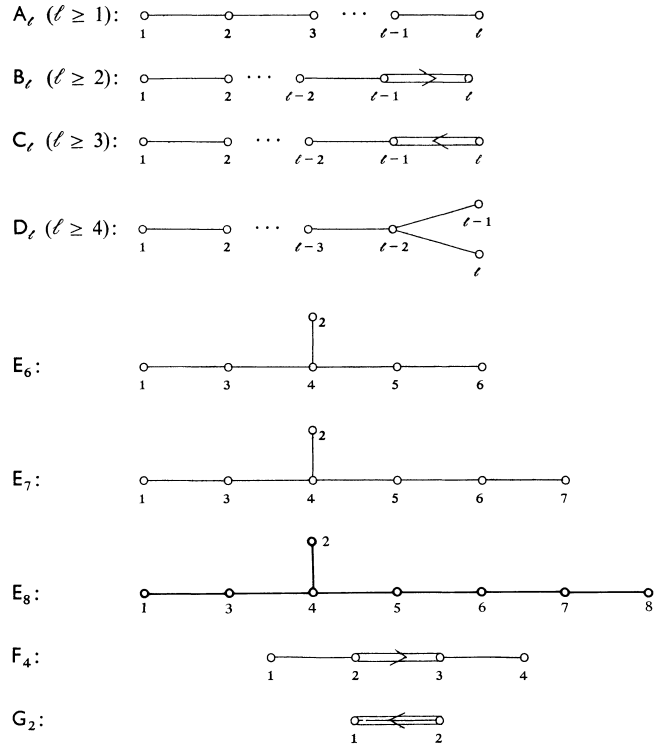
\includegraphics[scale=0.5]{rootsystems.png}
    \end{center}
    There exists a path of simple edges between any two roots of the same
    length. Thus, by $(1)$, they must be in the same $\mathcal{W}$-orbit.
    We know that $\mathcal{W}$ acts transitively on any of its orbits, thus we conclude.
    \item From Problem 1 on the previous pset, there is
    $w_0 \in \mathcal{W}$ which sends \emph{all} of $\Phi^+$ into $\Phi^-$. It is well-known that for any $\sigma \in 
    \mathcal{W}$, the length of $\sigma$ is the number of positive roots which are sent 
    to negative roots. So clearly this $w_0$ 
    is of maximal length, and it's length is $|\Phi^+| = \frac12 |\Phi|$.
    \item 
    Any positive root 
    $\alpha \in \Phi^+$ is sent into $\Phi^-$ by \textit{exactly one of} $w$ and $w_0w$. 
    Thus $\ell(w) + \ell(w_0w) = |\Phi^+| = \ell(w_0)$, as desired.
\end{enumerate}



\section{Nilpotent and Borel Subalgebras}

\begin{prob*}
Let $\mathfrak g$ be a semisimple Lie algebra. Let $\mathfrak h$ be a Cartan subalgebra of $\mathfrak g$. Let $\Phi$ be the set of $\mathfrak h$ roots with a base $\Delta$.
\begin{enumerate}
    \item Set $\mathfrak n_+ := \bigoplus_{\alpha \in \Phi_+} \mathfrak g_\alpha$. Prove that $n_+$ is nilpotent.
    \item Set $\mathfrak b := \mathfrak h + n_+$. Prove that $\mathfrak b$ is a Borel subalgebra, that is, it is a maximal solvable Lie subalgebra of $\mathfrak g$.
\end{enumerate}

\end{prob*}
\begin{enumerate}
    \item Recall that for any two roots $\alpha,\beta$ we have $[\mathfrak g_\alpha, \mathfrak g_\beta] \subseteq \mathfrak g_{\alpha + \beta}$; basically, if you iterate
    this too many times, you'll get a root which is not in $\Phi_+$, so the bracket will be zero.
    
    Specifically, let $\mathfrak n^{(1)} = \mathfrak n_+$ and $\mathfrak n^{(i+1)} = [\mathfrak g, \mathfrak n^{(i)}]$. It is clear that $\mathfrak n^{(i)} = \bigoplus_{c \in \Phi_+^n} \mathfrak g_c$ where $\Phi_+^n$ is the set of all sums of $n$ positive roots.
    Since $\Phi$ is finite, there exists some $N$ such that $\Phi_+^N = \emptyset$, so $\mathfrak n^{(N)} = \{0\}$ and $\mathfrak n_+$ is nilpotent.
    \item This time, let $\mathfrak b^{(0)} = \mathfrak b$ and $\mathfrak b^{(i+1)} = [\mathfrak b^{(i)}, \mathfrak b^{(i)}]$. 
    
    I claim $\mathfrak b^{(1)} = [\mathfrak b, \mathfrak b]\subset \mathfrak n_+$.
    This is completely obvious; $[\mathfrak h + \mathfrak n_+, \mathfrak h + \mathfrak n_+]$ contains $[\mathfrak h, \mathfrak h]$, which is zero, $[\mathfrak h, \mathfrak n_+]$, which is contained in $\mathfrak n_+$, and $[\mathfrak n_+, \mathfrak n_+]$, which is contained in $\mathfrak n_+$.

    Thus $\mathfrak b^{(1)} \subseteq \mathfrak n_+$ is nilpotent; then of course $\mathfrak b$ is solvable.
    
    To show $\mathfrak b$ is maximal, suppose for contradiction $\mathfrak m$ is a solvable subalgebra of $\mathfrak g$ containing $\mathfrak b$; then $\mathfrak m$ must contain some root space $\mathfrak g_{-\alpha}$ for some $\alpha \in \phi^+$.
    Then, $\mathfrak m$ contains $g_{\alpha}$ and $g_{-\alpha}$.
    
    This lets us pick elements $e \in \mathfrak g_\alpha, f \in \mathfrak g_{-\alpha}, h = [e,f]$ which span a $\mathfrak{sl}_2$ subalgebra of $\mathfrak m$.
    
    Since $\mathfrak{sl}_2$ is simple, $\mathfrak m$ cannot be solvable, and we're done.
\end{enumerate}



\section{Center of $U(\mathfrak{sl}_2)$}

\begin{prob*}
Let $U(\mathfrak{sl}_2)$ be the universal enveloping algebra of $\mathfrak{sl}_2$ and $e, h, f$ be the standard basis. Prove that
\[C = ef + fe + \frac{1}{2} h^2\]
is in the center of $U(\mathfrak{sl}_2)$.

\end{prob*}
We check the commutation relations.
\begin{align*}
    [C, e] &= [ef + fe + \frac{1}{2} h^2, e] \\
    % &= [ef, e] + [fe, e] + \frac12 [ h^2, e] \\
    &= [f,e^2] + \frac12 (h[h,e] + [h,e]h) \\
    &= [f,e]e + e[f,e] + eh +he\\
    &= -he - eh + eh + he = 0\\
    [C, f] &= [ef + fe + \frac{1}{2} h^2, f] \\
    % &= [ef, f] + [fe, f] + \frac12 [ h^2, f] \\
    &= [e,f^2] + \frac12 (h[h,f] + [h,f]h) \\
    &= [e,f]f + f[e,f] -hf - fh\\
    &= hf + fh - hf - fh = 0\\
    [C, h] &= [ef + fe + \frac{1}{2} h^2, h] \\
    % &= [ef, h] + [fe, h]  \\
    &= [e,h]f + e[f,h] + [f,h]e + f[e,h] \\
    &= -2ef + 2ef + 2fe - 2fe = 0
\end{align*}

\end{document}